\chapter{Several Key points}
\section{Morphological Box}
Create a morphological box, which is a way of creative thinking in functions and sequence of work steps.
\begin{table}[ht]
	\centering
	\begin{tabular}{lp{0.2\linewidth}p{0.12\linewidth}p{0.12\linewidth}p{0.12\linewidth}p{0.12\linewidth}p{0.12\linewidth}}\toprule
		\multirow{2}{*}{} & \multirow{2}{*}{Sub functions} & \multicolumn{5}{l}{Solutions of the sub functions}\\\cmidrule{3-7}
		& & 1 & 2 & 3 & 4 & 5\\
		\midrule
		A & Sub function 1 & \textbf{solution A1 (1) (3)} & solution A2 & solution A3 & &\\
		B & Sub function 2 & solution B1 (1) (2) (3) & solution B2 (2) & \textbf{solution B3 (2)} & \multicolumn{2}{l}{solution B45} \\
		C & Sub function 2 &  & solution C2 (2)  & \textbf{solution C3 (1)} & & solution C5 \\\bottomrule
	\end{tabular}
	\caption{A morphological box with 3 concept variants}
\end{table}\\
Legend\\
(1) = thermal solution\\
(2) = mechanical solution\\
(3) = MEM solution

For each bold option, if there are many concept variants, see Table \ref{subsub2}. In this example, we choose sub function B1 as the optimal solution with 3 variants. If the table does not describe fully or the sub function needs dividing into subgroups, see Table \ref{subsub1}.

\begin{table}[ht]
	\centering
	\begin{tabular}{lp{0.2\linewidth}p{0.2\linewidth}p{0.2\linewidth}p{0.2\linewidth}}\toprule
		\multirow{2}{*}{} & \multirow{2}{*}{Sub functions} & \multicolumn{3}{l}{Solutions of the sub functions}\\\cmidrule{3-5}
		& & 1 & 2 & 3\\
		\midrule
		A & Sub function 1 & Thermal treatment & MEM treatment & \\
		&  &   & MEM 1  & MEM 2 \\
		B & ... &  &  &   \\\bottomrule
	\end{tabular}
	\caption{A morphological box with 3 concept variants}
	\label{subsub1}
\end{table}
When calling a solution in Table \ref{subsub1}, we call it position + name of the sub solution (e.g. A2 MEM 1)
\begin{table}[ht]
	\centering
	\begin{tabular}{lp{0.2\linewidth}p{0.2\linewidth}p{0.2\linewidth}p{0.2\linewidth}}\toprule
		\multirow{2}{*}{} & \multirow{2}{*}{Sub functions} & \multicolumn{3}{l}{Solutions of the sub functions}\\\cmidrule{3-5}
		& & 1 & 2 & 3\\
		\midrule
		B & Sub function 2 & & & \\
		Ba & Type  &  Simple & Complex  & Mixed \\
		Bb & Shape & Round & Square & Triangle  \\
		Bc & Size $ \unitp{m} $  & 7x2 & 2x2 & 3x5 \\\bottomrule
	\end{tabular}
	\caption{A morphological box with 3 concept variants}
	\label{subsub2}
\end{table}

\section{Evaluation Table}
Many evaluation tables are developed in the industry (e.g VDI 2222, VDI 2225). Search for the sheet form on the internet, consult with your supervisor/customer for further information before using it.
\begin{figure}[ht]
	\centering
	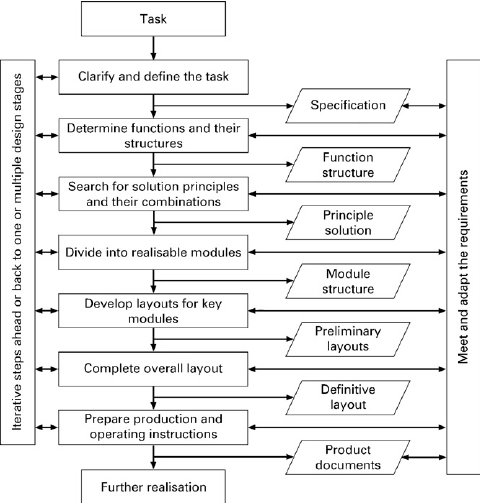
\includegraphics{images/01}
	\caption{A figurative example of VDI 2222}
	\label{fig:01}
\end{figure}

General points to remember to make better decisions:
\begin{itemize}
	\item Use consecutively (following one another).
	\item Every table should have its own acronym since turning pages is avoided.
	\item Simple points are related to almost other categories. Examples:\\
	Parallel point values: load carrying $ \uparrow \Rightarrow $ beneficial $ \uparrow \Rightarrow $ simple point $ \uparrow $\\
	Opposite point values: self-weight $ \uparrow \Rightarrow $ bad $ \downarrow \Rightarrow $ simple point $ \downarrow $
	\item Think as a user/customer, not a manufacturer.
\end{itemize}